\begin{frame}{Challenge 1 - Signal to background separation}
\begin{block}{Problem 1}
    \begin{itemize}
        \item Separation of signal to background
        \item Signal: $\tW\_DR$, $\tW\_DS$
        \item Background: \ttbar
    \end{itemize}
\end{block}
\begin{block}{Classic approach}
    Applying cuts
\end{block}
\begin{block}{Alternative}
    \begin{itemize}
        \item Machine Learning
        \item In particular: Classifying neural network
    \end{itemize}
\end{block}
\end{frame}

\begin{frame}[c]
\begin{center}
\Huge Artificial neural network
\end{center}
\end{frame}

\begin{frame}{Neural Networks - Processing information}
\begin{columns}
\quad
    \begin{column}{0.45\textwidth}
    \begin{block}{Human senses}
    \begin{itemize}
        \item Extract relevant information
        \item Not possible for machines
    \end{itemize}
    \end{block}
    %
    \begin{block}{Human brain}
        \begin{itemize}
            \item Web of neuron cells
            \item A neuron cell takes input from other cells
            \item Combination of signals creates a result
        \end{itemize}
    \end{block}
    %
    \end{column}
    \quad
    \begin{column}{0.45\textwidth}
    %
    \begin{block}{Input variables}
    \begin{itemize}
        \item Preprocessed by human user
        \item {e.g.} kinematic variables of an event
    \end{itemize}
    \end{block}
    %
    \begin{block}{Net of nodes}
    \begin{itemize}
        \item Nodes are simple processors
        \item Connected by linear function (weight and bias)
        \item Combines input using an activation function
    \end{itemize}
    \end{block}
    \end{column}
\quad
\end{columns}
\end{frame}

\begin{frame}{Neural network structure}
\begin{figure}
\centering
\def\layersep{2.5cm}
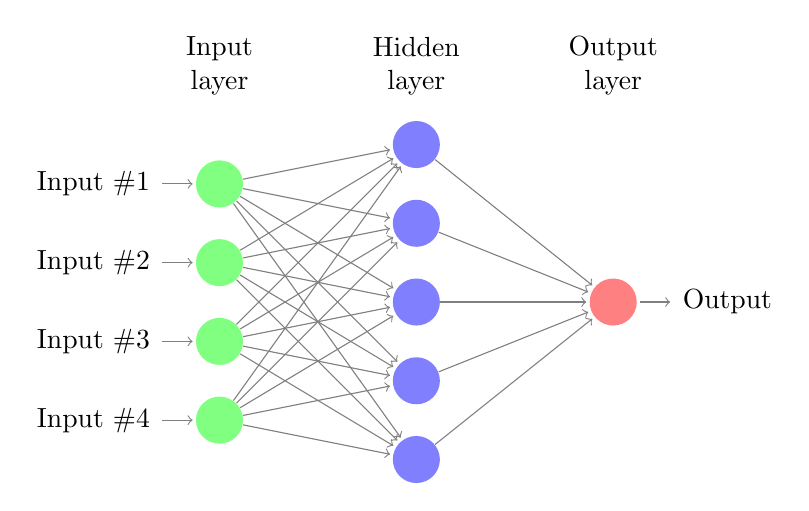
\begin{tikzpicture}[shorten >=1pt,->,draw=black!50, node distance=\layersep]
    \tikzstyle{every pin edge}=[<-,shorten <=1pt]
    \tikzstyle{neuron}=[circle,fill=black!25,minimum size=17pt,inner sep=0pt]
    \tikzstyle{input neuron}=[neuron, fill=green!50];
    \tikzstyle{output neuron}=[neuron, fill=red!50];
    \tikzstyle{hidden neuron}=[neuron, fill=blue!50];
    \tikzstyle{annot} = [text width=4em, text centered]
    % Draw the input layer nodes
    \foreach \name / \y in {1,...,4}
    % This is the same as writing \foreach \name / \y in {1/1,2/2,3/3,4/4}
        \node[input neuron, pin=left:Input \#\y] (I-\name) at (0,-\y) {};
    % Draw the hidden layer nodes
    \foreach \name / \y in {1,...,5}
        \path[yshift=0.5cm]
            node[hidden neuron] (H-\name) at (\layersep,-\y cm) {};
    % Draw the output layer node
    \node[output neuron,pin={[pin edge={->}]right:Output}, right of=H-3] (O) {};
    % Connect every node in the input layer with every node in the
    % hidden layer.
    \foreach \source in {1,...,4}
        \foreach \dest in {1,...,5}
            \path (I-\source) edge (H-\dest);
    % Connect every node in the hidden layer with the output layer
    \foreach \source in {1,...,5}
        \path (H-\source) edge (O);
    % Annotate the layers
    \node[annot,above of=H-1, node distance=1cm] (hl) {Hidden layer};
    \node[annot,left of=hl] {Input layer};
    \node[annot,right of=hl] {Output layer};
\end{tikzpicture}
\caption{\cite{NN_sketch}}
\label{fig:NN:tikz:sketch}
\end{figure}
\end{frame}

\begin{frame}{Neural Networks - Choosing the next step}
\begin{columns}
\quad
    \begin{column}{0.45\textwidth}
    \begin{block}{Evaluation of an action}
    \begin{itemize}
        \item Simple perceptions: pain, satisfaction
        \item Expected or desired outcome
    \end{itemize}
    \end{block}
    %
    \begin{block}{Deciding for a better action}
    \begin{itemize}
        \item Trial and error
        \item Learning from experience
    \end{itemize}
    \end{block}
    %
    \end{column}
    \quad
    \begin{column}{0.45\textwidth}
    %
    \begin{block}{Loss function}
    \begin{itemize}
        \item Supervised learning: compare to the desired outcome
        \item Loss is an estimator for a model's quality
    \end{itemize}
    \end{block}
    %
    \begin{block}{Optimisation}
    \begin{itemize}
        \item Propagate the impact of the parameters on the loss backwards
        \item Adjust parameters to achieve a model representing a smaller loss
    \end{itemize}
    \end{block}
    \end{column}
\quad
\end{columns}
\end{frame}

\begin{frame}{Challenge 2 - Sensitivity to systematic uncertainties}
\begin{block}{Problem 2}
    \begin{itemize}
        \item Minimal sensitivity to the systematic uncertainty
        \item Nominal: $\tW\_DR$, (\ttbar)
        \item Systematic: $\tW\_DS$
    \end{itemize}
\end{block}
\begin{block}{Presented solution}
   \begin{itemize}
       \item Addition of a second classifier for nominal to systematics separation
       \item Bad performance $\longrightarrow$ low sensitivity
   \end{itemize}
\end{block}
\begin{block}{Implementation}
    \begin{itemize}
        \item Feed output into a second net
        \item Iterative training
        \item Combined loss function $\longrightarrow$ Minimax problem
    \end{itemize}
\end{block}
\end{frame}

\begin{frame}{Adversarial neural network}
\vspace{-0.3cm}
    \begin{figure}
        \centering
        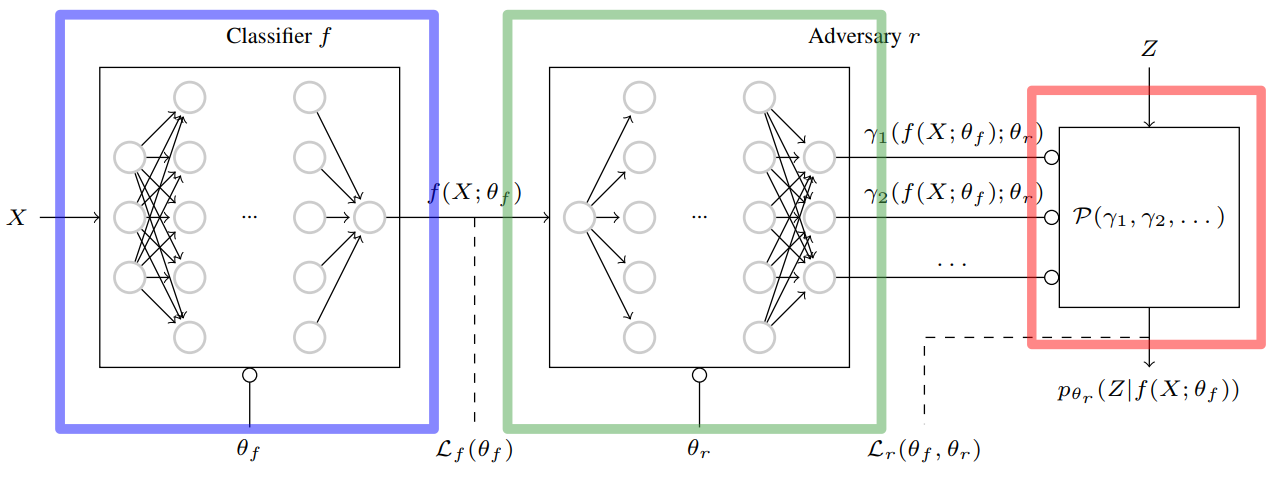
\includegraphics[width=\textwidth]{figures_theory/ANN_paper.png}
        \caption{\cite{Louppe:2016ylz}}
    \end{figure}
    \begin{equation*}
        \hfsetfillcolor{logo_blue!10}
        \hfsetbordercolor{logo_blue}
        \tikzmarkin{a}(0.3,-0.5)(-0.3,0.55)
        \mathbb{E}(\theta_f, \theta_r) = \mathcal{L}_f(\theta_f) - \lambda \mathcal{L}_r(\theta_f, \theta_r)
        \tikzmarkend{a}
    \end{equation*}
\end{frame}

\begin{frame}{Expected ANN losses}
    \begin{figure}
        \centering
        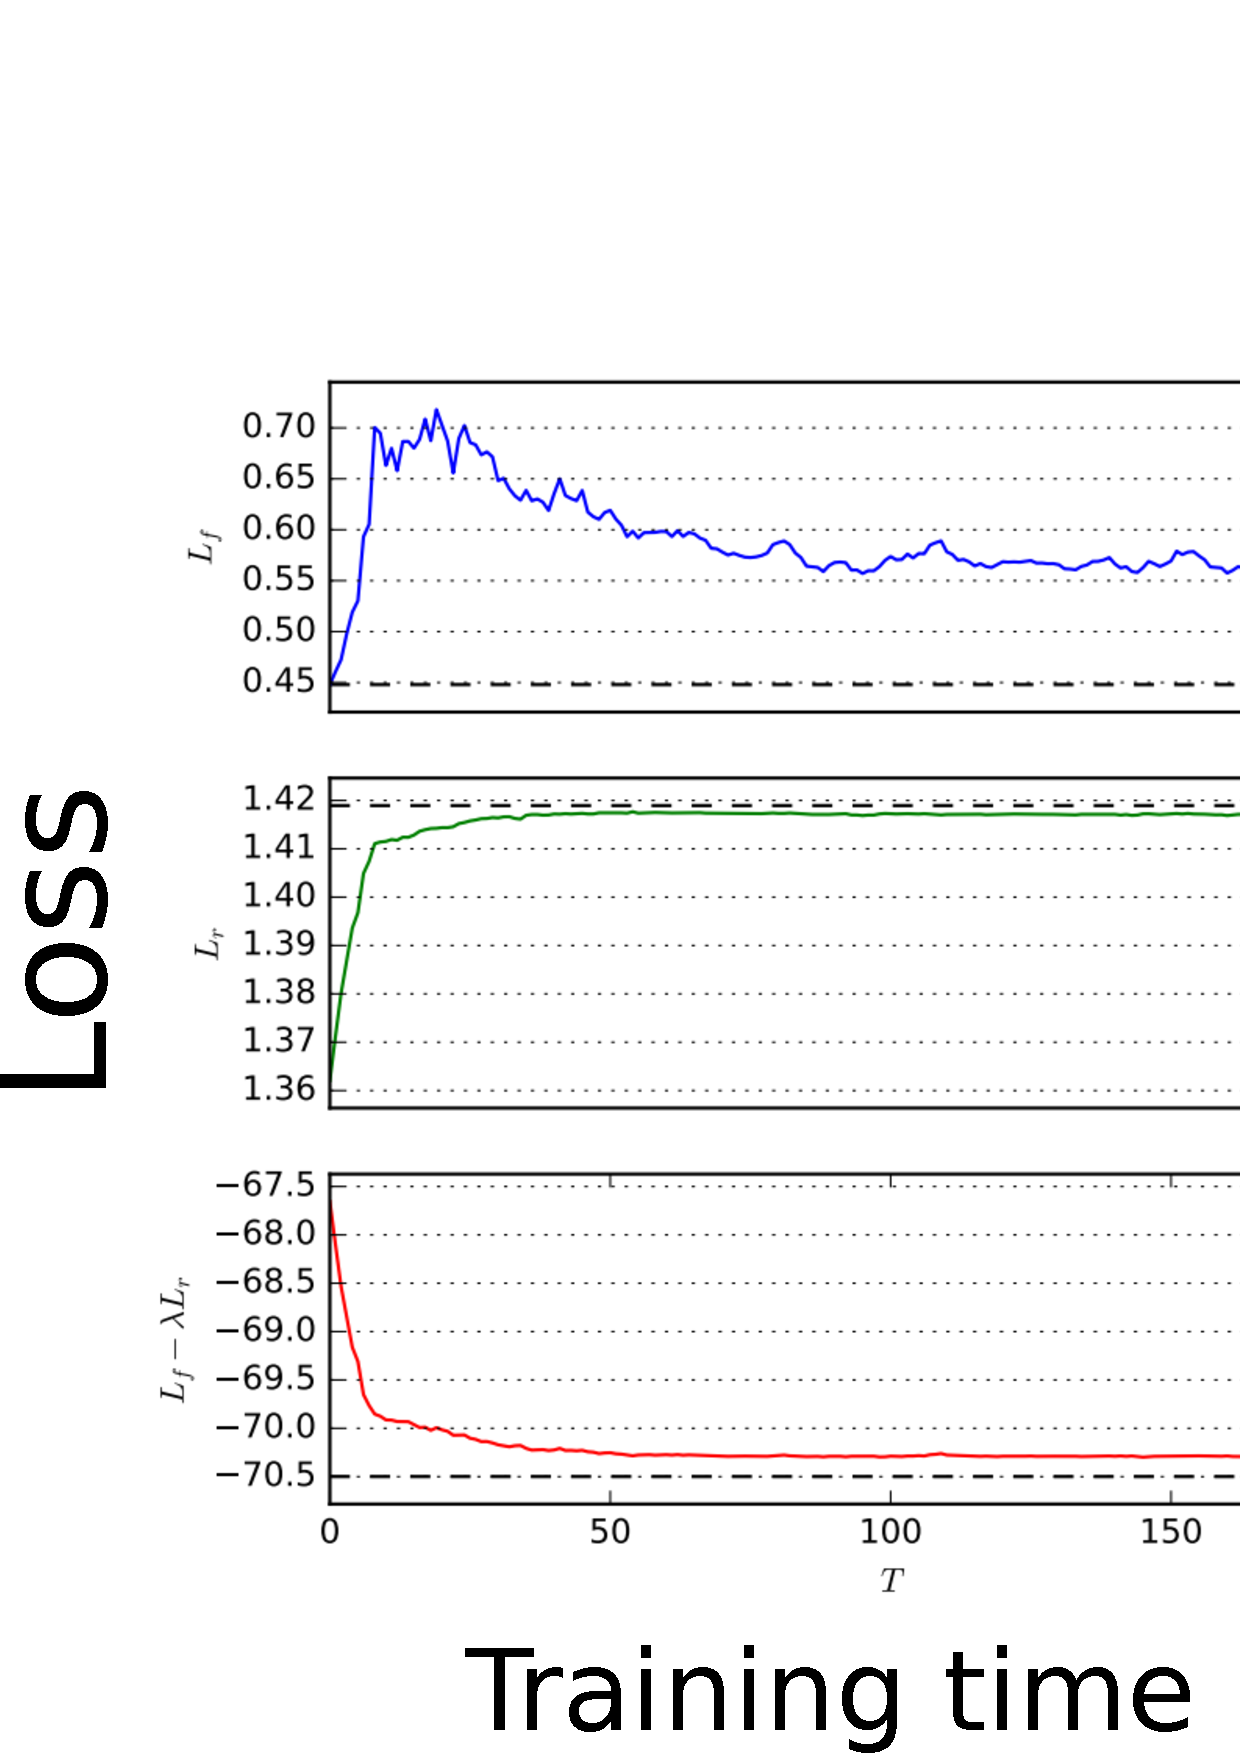
\includegraphics[width=0.8\textwidth]{figures_theory/losses_paper.png}
        \caption{\cite{Louppe:2016ylz}}
    \end{figure}
\end{frame}